\section{System Model}
%----------------------------------------------------------------------------------------%
\subsection{Network Model}
We denote as $\apSet \define \set{1,\dots,K}$ and $\mathcal{M} \define \set{1,\dots,M}$ Access Points (AP) and Edge Servers (ES) in our system respectively, as depicted in Fig. \ref{fig:system}.
Both the AP and ES side adopt the same timing mechanism with quantized \emph{time slot} lasting for $\tau$ second ($\tau \ll 1$).

\begin{figure}[ht]
    \centering
    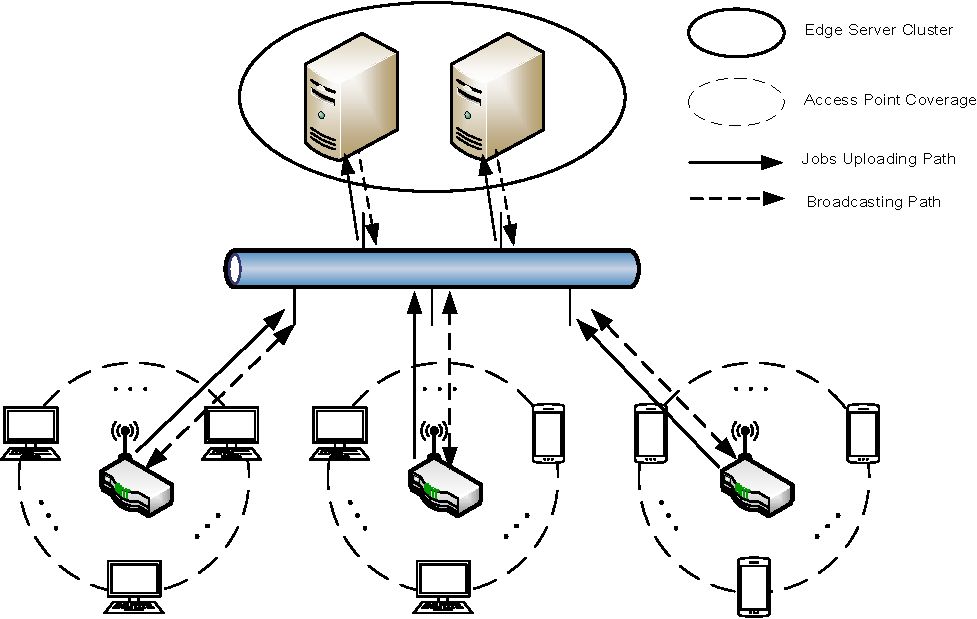
\includegraphics[width=0.45\textwidth]{system-model.pdf}
    \caption{The Illustration of MEC System Model}
    \label{fig:system}
\end{figure}

The User Equipment (UE) would offload the computation jobs on demand to the AP it connects.
We consider a list of types of jobs are supported on edge servers based on Virtual Machine (VM) resources, which is denoted as $\jSpace \define \set{1,\dots, J}$.
% which is obtained by statistics and denoted as $p_j \define \Pr\{\text{"j-type arrival"}\}$, where $\sum_{j\in\jSpace} p_j=1$.
Thus the job arrival process on $k$-th AP ($\forall k\in\apSet$) is compounded of the job arrivals from all UE connected, which follows the assumption as follows.
\begin{assumption}[Job Arrival Process for AP]
    The $j$-type job arrival distribution for $k$-th AP in one slot is denoted as $A_{k,j}(\tau)$, which is independent and identically distributed (i.i.d) over each time slot following Bernoulli distribution as $Bernoulli(\lambda_{k,j})$ ($\lambda_{k,j} > 0$).
    Thus average arrival rate of $j$-type jobs on $k$-th AP is $\mathbb{E}[A_{k,j}]=\lambda_{k,j}$.
\end{assumption}

The AP itself is assumed with no computation capability, and thus the jobs are further dispatched to the edge servers for processing.
The jobs arrival in each time slot on AP will be immediately dispatched to edge servers.
The corresponding uploading delay of dispatched process is \emph{un-predictable} over one AP-ES link, which is denoted as $U_{k,m}$ from $k$-th AP to $m$-th ES ($\forall k\in\apSet, \forall m\in\esSet$).
Without loss of generality, we assume $U_{k,m} \sim \Pr\{U_{k,m}\}$ in interval $[0, \Xi]$.

After arrival on edge servers, the jobs will join computation queue with the supported VM.
Each VM is considered running parallel without resource contention, and the jobs scheduling for each VM is with a single queue following \emph{FCFS} (First-Come-First-Serve).
{\color{red}The maximum queue length is set to discourage too many jobs pending on edge servers and is denoted as $L_Q$. The job submission over the limit will be rejected and announce the AP where the job is from.}

{\color{red}For jobs processing on edge servers, we adopt \emph{unrelated machines} assumption in \cite{tan-online}, where the job processing time on different servers are machine dependent and variant of resource or VM (virtual machine) constraints.
Moreover, we have $l_{m,j}$ to denote the processing time for $j$-type job on $m$-th edge serer following some distribution, whose largest processing time is bounded by $l_C$.}
For convenience, we assign type of jobs on edge servers which have no VM resource available with \emph{infinity} processing time, and this kind of dispatching possibility will be rejected at the AP side.

In the whole process, we care about the job completion time (JCT), which is the measurement of jobs from being uploaded until left the system. To optimize this measurement requires a fair dispatching decisions performance, a fairly scheduled and efficiently utilized system.
%----------------------------------------------------------------------------------------%

\subsection{Information-Sharing Broadcast Model}
In the decentralized system, a information sharing scheme is indispensable to guarantee a global-wise optimal policy than local greedy policy.
However, frequent information exchange would always introduce heavy network burden and communication latency is also a severe issue which causes stale information collection. So, an efficient scheme is needed to alleviate the communication burden and aware of the stale information impact.
In this article, the proposed sharing scheme leverage a common periodic broadcast which lasting for adjustable period $t_B \define N \times \tau$. More specifically, the broadcasting is applied in a loose synchronized way that all the nodes (including AP and ES) starts broadcasting at the same start and is received in that period due to the stochastic latency. We further adopt the following time denotation.
\begin{align}
    t_{i,n} = i \cdot T + n \cdot \tau, (i,n=0,1,2,\dots),
\end{align}
where $t_{i,n}$ denotes the $n$-th time slot in $i$-th interval w.r.t the start point. Especially, we denote as $t_{i} \define t_{i,0}$ as the start point of each broadcasting interval, which is called \emph{broadcast point}.
And the broadcast information is a sampling of the system status, for $i$-th \emph{broadcast point}, the composed broadcast information from all the AP and ES nodes is listed as follows.
\begin{itemize}
    \item Denote as
    $r^*(t_{i}) \define \set{ \vec{r}^{(k)}_{m,j}(t_i)|\forall k\in\apSet, m\in\esSet, j\in\jSpace }$
    the information AP cluster contains at $i$-th broadcast interval, where
    $\vec{r}^{(k)}_{m,j}(t_i) \triangleq \{ r^{(k)}_{m,j,\xi}(t_i)|\forall \xi=0,\dots,\Xi \}$
    denotes a series of counters recording the uploading time from $0$ to $\Xi$ of the $j$-type job from $k$-th AP to $m$-th ES.
    For each $k$-th AP ($\forall k\in\apSet$), it maintains its own information $\set{ \vec{r}^{(k)}_{m,j} | \forall m\in\esSet, j\in\jSpace}$;
    \item Denote as
    $Q^*(t_{i}) \triangleq \set{ Q_{m,j}(t_i)|\forall m\in\esSet,j\in\jSpace }$
    the information ES cluster contains at $i$-th broadcast interval, where
    $Q_{m,j}(t_i) \triangleq (l_{m,j}(t_i), \eta_{m,j}(t_i))$
    denotes the $j$-type jobs queue on $m$-th ES, while $l_{m,j}(t_i)$ denotes the queue length and $\eta_{m,j}(t_i)$ denotes the remaining time of the job in processing.
    The $m$-th ES ($\forall m\in\esSet$) maintains information $\set{ Q_{m,j}(t_i)|\forall j\in\jSpace }$.
\end{itemize}
Thus the composed broadcasting information at $t_i$ is denoted as:
\begin{align}
    \Obsv(t_i) \define
        \Brace{
            r^*(t_i),
            Q^*(t_i)
        }
\end{align}
And we notice that though $r^*(t_{i,n})$ and $Q^*(t_{i,n})$ also exists in each time slot, the observed information is only available of start of each interval via broadcast. The broadcasting shared information is actually a uniform sampling of the whole process.

As the broadcasting latency is random due to underlaid network, different AP nodes would receive partial broadcast information at different time slots in that interval. To alleviate the complexity of composition of randomness in a short time, here we only consider the \emph{maximum broadcast latency} when the node receives the last partial information.
We denote as $D^{(p)}_{k,k'}(t_i)$ the broadcast delay between $k'$-th AP and $k$-th AP ($\forall k,k'\in\apSet$), and $D^{(s)}_{k,m}(t_i)$ the broadcast delay between $m$-th ES and $k$-th AP ($\forall k\in\apSet,\forall m\in\esSet$).
Then we denote the latency for $k$-th AP receives broadcast information from other nodes (including all ES nodes and other AP nodes) as \emph{Maximum Broadcast Latency}.
\begin{definition}[Maximum Broadcast Latency]
    The maximum broadcast latency is the time when AP receives whole broadcast information with respect to the broadcast point. For $k$-th AP ($\forall k\in\apSet$) the latency for $i$-th interval is given as follows.
    \begin{align}
        D_{k}(t_i) \define \max\Paren{ \set{D^{(p)}_{k,k'}(t_i), D^{(s)}_{k,m}(t_i)|\forall k' \neq k \in\apSet, \forall m\in\esSet} }
    \end{align}
\end{definition}
Moreover, we assume that the broadcast interval is set a value that always larger than the maximum broadcast latency, i.e. $t_B > \hat{D}_k$ ($\forall k\in\apSet$), where $\hat{D}_k$ is the upper bound for $D_k$.

{\color{red}
    Due to the introduced periodic broadcasting design and the information receiving latency, this kind of system is inherent of the structure that decisions are always made with obsolete and partial information.
    This implies that: if any agents change its decision with respect to newly-arrival broadcast information, it will disturb other agents' decisions from cooperation due to different information of system states.
    Thus, it's unacceptable to update agents' policy only when the agents all come up with exactly same information.
}
        
In the problem formulation section, we will show that we could come up with better policy aware of the randomness of latency, and improve AP's policy in an iterative way.
Furthermore, with the help of algorithm design we could prove that our improved policy is with analytical performance bound under MDP framework.
%----------------------------------------------------------------------------------------%